% Created 2020-07-07 mar. 15:46
% Intended LaTeX compiler: pdflatex
\documentclass[11pt]{article}
\usepackage[utf8]{inputenc}
\usepackage[T1]{fontenc}
\usepackage{graphicx}
\usepackage{grffile}
\usepackage{longtable}
\usepackage{wrapfig}
\usepackage{rotating}
\usepackage[normalem]{ulem}
\usepackage{amsmath}
\usepackage{textcomp}
\usepackage{amssymb}
\usepackage{capt-of}
\usepackage{hyperref}
\usepackage{color}
\usepackage{mathpazo}
\author{Frédéric Santos}
\date{\today}
\title{pacmanUB : un pacman made in Bordeaux}
\hypersetup{
 pdfauthor={Frédéric Santos},
 pdftitle={pacmanUB : un pacman made in Bordeaux},
 pdfkeywords={},
 pdfsubject={},
 pdfcreator={Emacs 26.3 (Org mode 9.3.7)}, 
 pdflang={French}}
\begin{document}

\maketitle
\tableofcontents


\section{Présentation du logiciel}
\label{sec:orgdec5e37}
Pellentesque dapibus suscipit ligula.  Donec posuere augue in quam.  Etiam vel tortor sodales tellus ultricies commodo.  Suspendisse potenti.  Aenean in sem ac leo mollis blandit.  Donec neque quam, dignissim in, mollis nec, sagittis eu, wisi.  Phasellus lacus.  Etiam laoreet quam sed arcu.  Phasellus at dui in ligula mollis ultricies.  Integer placerat tristique nisl.  Praesent augue.  Fusce commodo.  Vestibulum convallis, lorem a tempus semper, dui dui euismod elit, vitae placerat urna tortor vitae lacus.  Nullam libero mauris, consequat quis, varius et, dictum id, arcu.  Mauris mollis tincidunt felis.  Aliquam feugiat tellus ut neque.  Nulla facilisis, risus a rhoncus fermentum, tellus tellus lacinia purus, et dictum nunc justo sit amet elit.

\textbf{Bold}
\emph{italic}
\uline{underline}
\texttt{verbatim}

\subsection{{\bfseries\sffamily TODO} Les développeurs}
\label{sec:orgb9c7125}
\label{sec-dev}
Nullam tempus.  

\section{Installation}
\label{sec:org608310b}
\subsection{Linux}
\label{sec:org170acce}
Nullam eu ante vel est convallis dignissim.  Fusce suscipit, wisi nec facilisis facilisis, est dui fermentum leo, quis tempor ligula erat quis odio.  Nunc porta vulputate tellus.  Nunc rutrum turpis sed pede.  Sed bibendum.  Aliquam posuere.  Nunc aliquet, augue nec adipiscing interdum, lacus tellus malesuada massa, quis varius mi purus non odio.  Pellentesque condimentum, magna ut suscipit hendrerit, ipsum augue ornare nulla, non luctus diam neque sit amet urna.  Curabitur vulputate vestibulum lorem.  Fusce sagittis, libero non molestie mollis, magna orci ultrices dolor, at vulputate neque nulla lacinia eros.  Sed id ligula quis est convallis tempor.  Curabitur lacinia pulvinar nibh.  Nam a sapien.

\subsection{{\bfseries\sffamily TODO} Mac OS}
\label{sec:org016725c}
Pellentesque dapibus suscipit ligula.

\subsection{Windows}
\label{sec:org8adb8f2}
\subsubsection{Windows 7}
\label{sec:org7bf8ba8}
\begin{itemize}
\item Télécharger
\item Décompresser
\item Installer
\end{itemize}

\subsubsection{Windows 10}
\label{sec:org106850d}
\begin{enumerate}
\item Télécharger
\item Décompresser
\item Installer
\end{enumerate}

\section{Comparaison avec d'autres logiciels}
\label{sec:org71f7734}
Voici la concurrence :

\begin{table}[htbp]
\centering
\begin{tabular}{llr}
\hline
Logiciels & OS & Prix\\
\hline
pacmanUB & Tous les OS & 19\\
pacTux & Linux & 0\\
iPac & Mac OS & 99\\
pacWin & Windows & 29\\
\hline
Collection complète &  & 147\\
\hline
\end{tabular}
\caption{Les différents Pacman sur le marché. \label{tab-concur}}

\end{table}

\section{L'avis de la presse}
\label{sec:orga147540}
Notre jeu a été testé sur le site web \href{https://www.canardpc.com}{Canard PC}.

Si vous avez connaissance d'autres tests, vous pouvez nous écrire à l'adresse qui figure en section \ref{sec-dev}.

\section{Captures d'écran}
\label{sec:org5e0747f}
Voici des images du jeu en figure \ref{fig-capture}.

\begin{figure}[htbp]
\centering
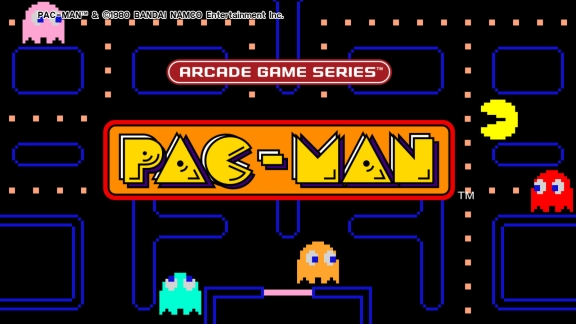
\includegraphics[width=.9\linewidth]{./pacman.jpg}
\caption{pacmanUB en action ! \label{fig-capture}}
\end{figure}

\section{Algorithme}
\label{sec:org8f7fcfe}
Les déplacements des fantômes obéissent à une formule très compliquée : \(\cos(\xi + \pi/6) = \theta\).
\end{document}